

\documentclass{beamer}

\mode<presentation> {

\usetheme{Boadilla}

\setbeamertemplate{footline}[page number] % To replace the footer line in all slides with a simple slide count uncomment this line

\setbeamertemplate{navigation symbols}{} % To remove the navigation symbols from the bottom of all slides uncomment this line
}
\usepackage[utf8]{inputenc}
\usepackage[brazil]{babel}
\setbeamercolor{alerted text}{fg=blue}
\usepackage{subfig}
\usepackage{amsmath}
\usepackage{graphicx} % Allows including images
\usepackage{booktabs} % Allows the use of \toprule, \midrule and \bottomrule in tables

%----------------------------------------------------------------------------------------
%	TITLE PAGE
%----------------------------------------------------------------------------------------

\title[ ]{\textbf{Modelo de otimização mutiobjetivo para adequação de embarcações de alta velocidade}\\Apresentação Parcial PAIC 2017/2018} % The short title appears at the bottom of every slide, the full title is only on the title page

\author[L.E.F.B]{Luiz Eduardo Fernandes Bentes, Renata da Encarnação Onety} % Your name
\institute[UEA] % Your institution as it will appear on the bottom of every slide, may be shorthand to save space
{
Universidade do Estado do Amazonas \\ Escola Superior de Tecnologia -- EST\\ Manaus - Amazonas - Brasil\\ % Your institution for the title page
\medskip
\textit{\{lefb.eng,ronety\} @uea.edu.br} % Your email address
}
\date{\today} % Date, can be changed to a custom date

\begin{document}

\begin{frame}
\titlepage % Print the title page as the first slide
\end{frame}

\begin{frame}
\frametitle{Overview}
\tableofcontents
\end{frame}

%------------------------------------------------
\section{Introdução} 
%------------------------------------------------
\begin{frame}
 \tableofcontents[ 
    currentsubsection, 
    hideothersubsections, 
    sectionstyle=show/shaded
    ] 
\end{frame}
%-------------------------------------------------
\begin{frame}
\frametitle{Introdução}
\begin{itemize}
	\item Para prestar socorro à população em atendimentos de urgência e emergência em saúde, as regiões sem acesso terrestre contam com o serviço de SAMU Fluvial.
	\item Atendimento similar às ambulâncias terrestres.
\end{itemize}

\begin{figure}[h]
	\centering
	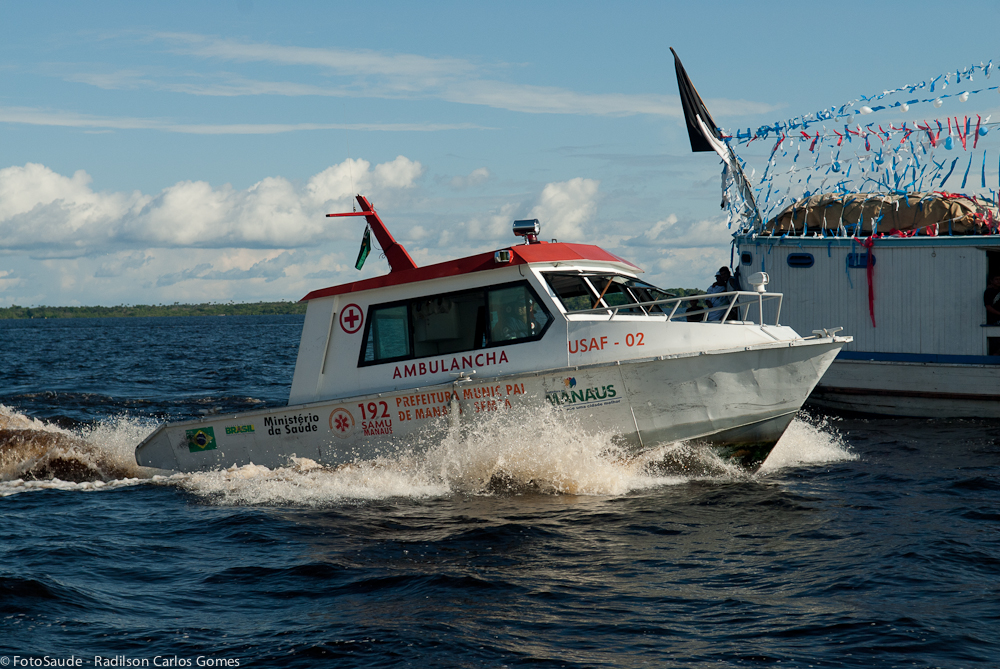
\includegraphics[scale=0.7]{samu17}
	\caption{Ambulâncias Fluviais\\Fonte: FotoSaúde}
	\label{fig:ambulancha}
\end{figure}

\end{frame}

%------------------------------------------------
\section{Justificativa}
%------------------------------------------------
\begin{frame}
\tableofcontents[ 
    currentsubsection, 
    hideothersubsections, 
    sectionstyle=show/shaded
    ] 
\end{frame}
%-------------------------------------------------
\begin{frame}
\frametitle{Justificativa}
\begin{itemize}
\item Atributos em relação à integridade estrutural devem ser atendidos
\item Modelo atual representa um projeto desenvolvido para navegação marítima.
\item Propor modelo que possa atender a população da melhor maneira possível  
\end{itemize}
\end{frame}
%-------------------------------------------------

\begin{frame}
\frametitle{Justificativa}
\begin{itemize}
	\item \alert{Atributos em relação à integridade estrutural devem ser atendidos}
	\begin{itemize}
		\item Estrutura suporte as cargas
		\item Ergonomia e bem-estar da tripulação
	\end{itemize}
	\item Modelo atual representa um projeto desenvolvido para navegação marítima.
	\item Propor modelo que possa atender a população da melhor maneira possível  
\end{itemize}
\end{frame}

%-------------------------------------------------
\begin{frame}
\frametitle{Justificativa}
\begin{itemize}
	\item Atributos em relação à integridade estrutural devem ser atendidos
	\item \alert{Modelo atual representa um projeto desenvolvido para navegação marítima}
	\begin{itemize}
		\item Distancia-se da realidade Fluvial do Amazonas
		\item Diferença da via e variações da água contribuem no desconforto
	\end{itemize}
	\item Propor modelo que possa atender a população da melhor maneira possível  
\end{itemize}
\end{frame}
%-------------------------------------------------
\begin{frame}
\frametitle{Justificativa}
\begin{itemize}
	\item Atributos em relação à integridade estrutural devem ser atendidos
	\item Modelo atual representa um projeto desenvolvido para navegação marítima
	\item \alert{Propor modelo que possa atender a população da melhor maneira possível}  
\end{itemize}
\end{frame}

%------------------------------------------------
\section{Objetivos}
%------------------------------------------------
\begin{frame}
\tableofcontents[ 
    currentsubsection, 
    hideothersubsections, 
    sectionstyle=show/shaded
    ] 
\end{frame}
%-------------------------------------------------
\begin{frame}
\frametitle{Objetivos}
\large
\begin{block}{Objetivo Geral}
Propor um modelo de otimização multiobjetivo baseado em Algoritmos Evolutivos para auxiliar no projeto de embarcações de alta velocidade, como as ambulanchas.
\end{block}
\pause
\begin{block}{Objetivos Específicos}
\begin{itemize}
\item Identificar métodos de construção de embarcações;
\item Desenhar o casco da embarcação através dos parâmetros de construção;
\item Propor algoritmo evolutivo para a otimização de variáveis do projeto
\item Implementar uma ferramenta computacional com interface amigável para auxiliar os projetistas desse tipo de embarcação.
\item Sugerir modelos de embarcações otimizadas.
\end{itemize}

\end{block}
\end{frame}
%-------------------------------------------------
\begin{frame}
\frametitle{Objetivos}
\large
\begin{block}{Objetivo Geral}
	Propor um modelo de otimização multiobjetivo baseado em Algoritmos Evolutivos para auxiliar no projeto de embarcações de alta velocidade, como as ambulanchas.
\end{block}
\begin{block}{Objetivos Específicos}
	\begin{itemize}
		\item \alert{Identificar métodos de construção de embarcações;}
		\item \alert{Desenhar o casco da embarcação através dos parâmetros de construção;}
		\item Propor algoritmo evolutivo para a otimização de variáveis do projeto
		\item Implementar uma ferramenta computacional com interface amigável para auxiliar os projetistas desse tipo de embarcação.
		\item Sugerir modelos de embarcações otimizadas.
	\end{itemize}
	
\end{block}
\end{frame}
%------------------------------------------------
\begin{frame}
\begin{figure}[h]
	\centering
	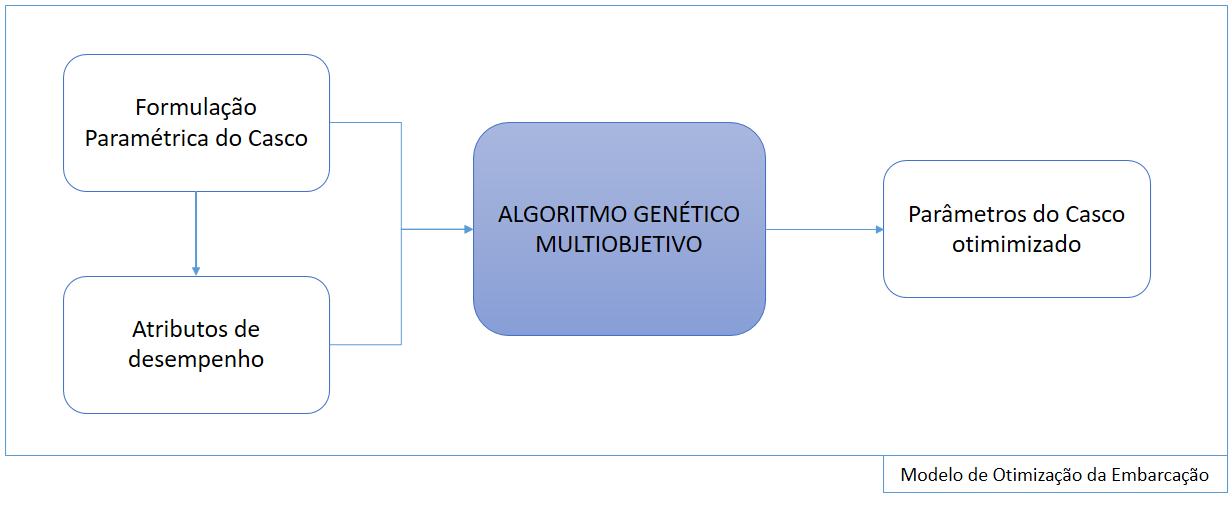
\includegraphics[scale=0.37]{img}
	\caption{Modelo proposto para otimização da embarcação}
	\label{fig:modelo}
\end{figure}
\end{frame}
%------------------------------------------------
\section{Fundamentação Teórica}
%------------------------------------------------
\begin{frame}
\tableofcontents[ 
    currentsubsection, 
    hideothersubsections, 
    sectionstyle=show/shaded
    ] 
\end{frame}
%-------------------------------------------------

\subsection{Curvas B-spline}
\begin{frame}{Curvas B-spline}
\begin{itemize}
\item Comumente usada na Engenharia Naval
\item Trata-se de uma curva formada por partes polinomiais chamadas \textbf{Partes de Bézier}
\item Polígono de Controle e Algoritmo de Interpolação (Algoritmo de De Boor)
\end{itemize}

\begin{block}{Definição}
	\begin{equation}
		S(u) = \sum_{j = 0}^{n} {P_j B_j^n(u)} = \sum_{j = 0}^{n} {X_j B_j^n(u),Y_j B_j^n(u)}
	\end{equation}
\end{block}

\begin{figure}[h]
	\centering
	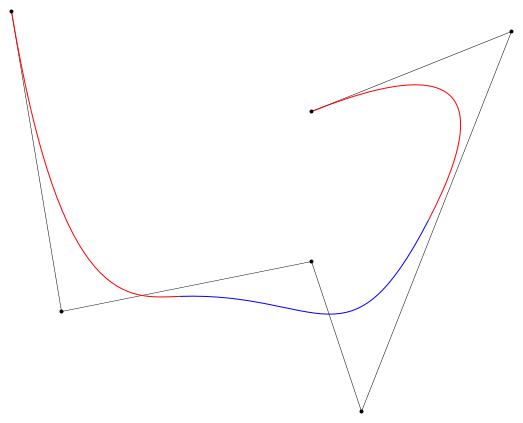
\includegraphics[scale=0.15]{bspline}
	\caption{Exemplo de Curva B-spline}
	\label{fig:bspline}
\end{figure}
\end{frame}

%------------------------------------------------

\subsection{Geração Paramétrica de Cascos de Planeio}
\begin{frame}{Geração Paramétrica de Cascos de Planeio}
\begin{itemize}
	\item Artigo de F. Pérez-Arribas. \cite{perez2006automatic}
	\item Método para desenvolver a curva apenas utilizando os parâmetros de construção do barco. \cite{morales2013flow}
	\item Dado os \textbf{Parâmetros da Embarcação}, as \textbf{Restrições das Curvas} e \textbf{Equação da Curva de B-spline} pode-se determinar os pontos de controle.
	
\end{itemize}

\begin{figure}[h]
	\centering
	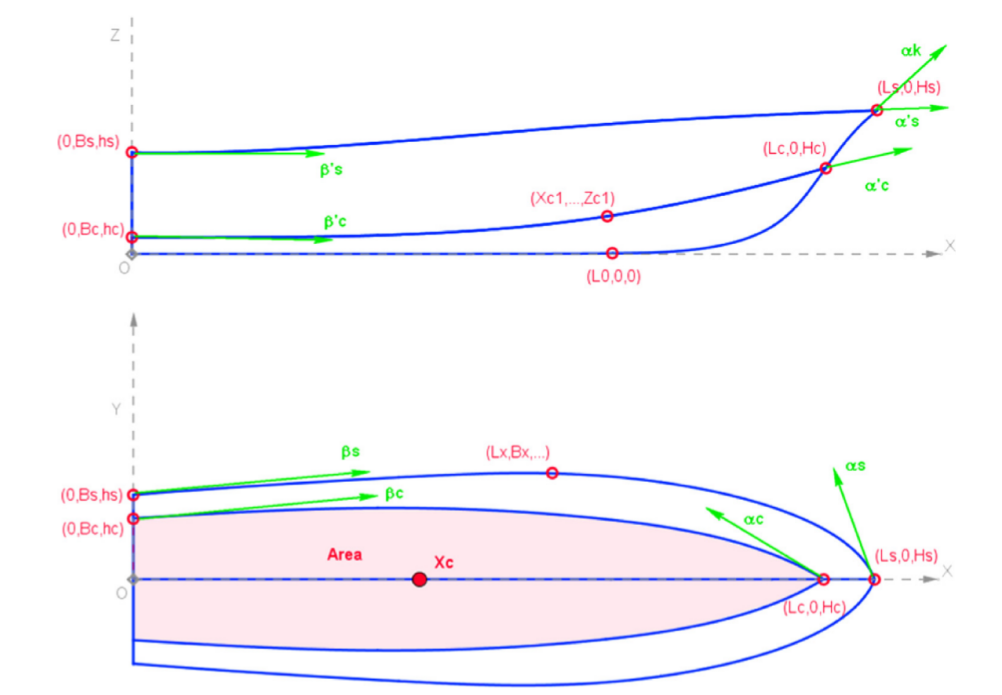
\includegraphics[scale=0.2]{vistas}
	\caption{Exemplo das vistas geradas utilizando o método de F.Pérez-Arribas}
	\label{fig:bspline}
\end{figure}
\end{frame}

%------------------------------------------------

\subsection{Python + OpenGL}
\begin{frame}
\frametitle{Python + OpenGL}
\begin{itemize}
	\item OpenGL é uma API livre utilizada na computação gráfica
	\item GLUT - Interface para desenho das curvas. 
\end{itemize}

\begin{figure}[h]	
\centering

\includegraphics[width=4cm]{Python}
\qquad

\includegraphics[width=4cm]{logoopengl}
\end{figure}

\end{frame}    

%------------------------------------------------
\section{Resultados Parciais}
%------------------------------------------------
\begin{frame}
\tableofcontents[ 
    currentsubsection, 
    hideothersubsections, 
    sectionstyle=show/shaded
    ] 
\end{frame}
%-------------------------------------------------
\subsection{Vista Lateral}
\begin{frame}{Vista Lateral}
\begin{itemize}
	\item Formada por 3 curvas principais:
		\begin{itemize}
			\item Linha Central
			\item Linha \textit{Sheer}
			\item Linha \textit{Chine}
		\end{itemize}
\end{itemize}
\begin{figure}[h]
	\centering
	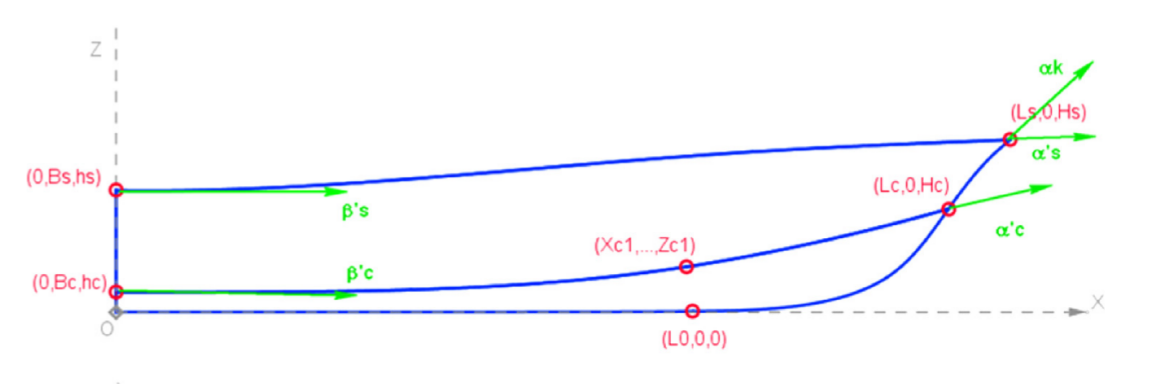
\includegraphics[scale=0.4]{vistalateral}
	\caption{Exemplo de Curva B-spline}
	\label{fig:central}
\end{figure}
\end{frame}
%-----------------------------------------------
\begin{frame}{Vista Lateral - Central}
\begin{block}{Linha Central}
	\begin{equation}
		\centering
		c(u) = B^3_0K_0 +B^3_1P_1+B^3_2P_2+B^3_3K_2
	\end{equation}
\end{block}
\begin{itemize}
	\item Restrições:
	\begin{enumerate}
		\item $c'_z(0) = 0$
		\item $c'_z(1) = tg(a_k)$
		\item $c(u*) = K_1$
	\end{enumerate}
	\item Tal que $u* = \dfrac{Dist(K_0,K_1)^k}{Dist(K_0,K_1)^k + Dist(K_1,K_2)^k}$
	\item Com as restrições acima podemos montar a matriz:
\end{itemize}
	
\begin{bmatrix}
$0$ & $1$ & $0$ & $0$ \\
$0$ & $0$ & $-tg(a_k)$ & $1$ \\
$B^3_1(u*)$ & $0$ & $B^3_2(u*)$ & $0$ \\
$0$ & $B^3_1(u*)$ & $0$ & $B^3_2(u*)$
\end{bmatrix}
\begin{bmatrix}
$XP_1$\\
$ZP_1$\\
$XP_2$\\
$ZP_2$
\end{bmatrix}
=
\begin{bmatrix}
$0$\\
$H_s - tg(a_k).L_s$\\
$L_c- B^3_0(u*)L_0$\\
$H_c - B^3_3(u*).H_s$
\end{bmatrix}

\end{frame}
%----------------------------------------------
\begin{frame}{Vista Lateral - Central}
\begin{figure}[h]	
	\centering
	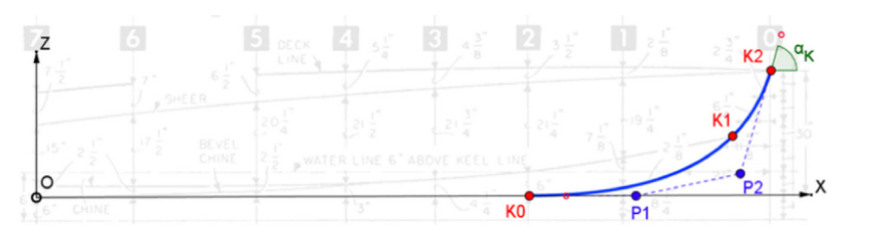
\includegraphics[width=9cm]{centerline}
\end{figure}
\end{frame}

%----------------------------------------------
\begin{frame}{Vista Lateral - Central}
\begin{figure}[h]	
	\centering
	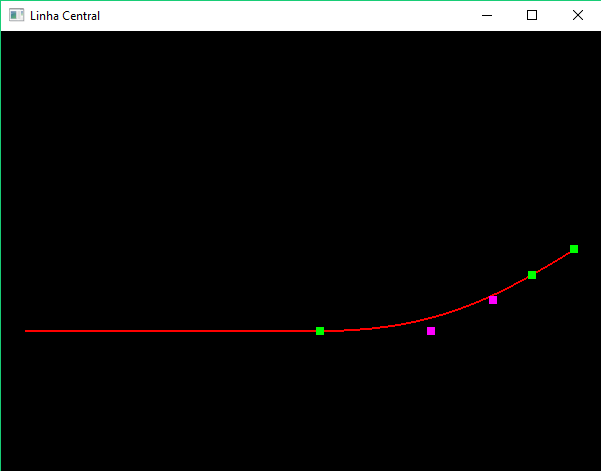
\includegraphics[width=9cm]{linhacentral}
\end{figure}
\end{frame}
%----------------------------------------------
\begin{frame}{Vista Lateral - Sheer}
\begin{block}{Linha Sheer}
	\begin{equation}
	\centering
	s_L(u) = B^2_0S'_0 +B^2_1P_1+B^2_2S'_2
	\end{equation}
\end{block}
\begin{itemize}
	\item Restrições:
	\begin{enumerate}
		\item $s_L(0) = S'_0$
		\item $s_L(1) = S'_2$
		\item $s'_L(0) = tg(B'_s)$
		\item $s'_L(1) = tg(a'_s)$
	\end{enumerate}
	\item Com as restrições acima podemos montar a matriz:
\end{itemize}

$	
\begin{bmatrix}
	$tg(B'_s)$ & $-1$ \\
	$-tg(a'_s)$ & 1 \\
\end{bmatrix}
\begin{bmatrix}
	$XP_1$\\
	$ZP_1$
\end{bmatrix}
=
\begin{bmatrix}
	$-h_s$\\
	$H_s - tg(a'_s).L_s$
\end{bmatrix}
$
\end{frame}
%----------------------------------------------
\begin{frame}{Vista Lateral - Sheer}
\begin{figure}[h]	
	\centering
	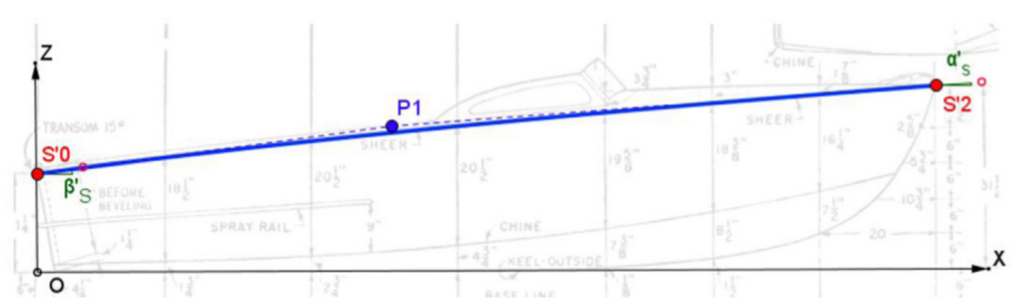
\includegraphics[width=9cm]{sheerline}
\end{figure}
\end{frame}

%----------------------------------------------
\begin{frame}{Vista Lateral - Sheer}
\begin{figure}[h]	
\centering
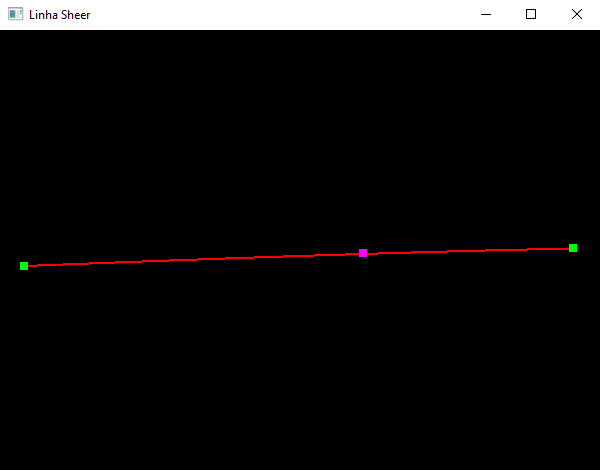
\includegraphics[width=9cm]{linhasheer}
\end{figure}
\end{frame}
%----------------------------------------------

\begin{frame}{Vista Lateral - Chine}
\begin{block}{Linha Chine}
	\begin{equation}
	\centering
	c_L(u) = B^3_0C'_0 +B^3_1P_1+B^3_2P_2+B^3_3C'_2
	\end{equation}
\end{block}
\begin{itemize}
	\item Restrições:
	\begin{enumerate}
		\item $c'_L(0) = tg(B'_c)$
		\item $c'_L(1) = tg(a_c)$
		\item $c_L(u*) = C_1$
	\end{enumerate}
	\item Tal que $u* = \dfrac{Dist(K_0,K_1)^k}{Dist(K_0,K_1)^k + Dist(K_1,K_2)^k}$
	\item Com as restrições acima podemos montar a matriz:
\end{itemize}	
$
\begin{bmatrix}
	$-tg(B'_c)$ & 1 & 0 & 0 \\
	0 & 0 & $-tg(a'_c)$ & 1 \\
	$B^3_1(u*)$ & 0 & $B^3_2(u*)$ & 0 \\
	0 & $B^3_1(u*)$ & 0 &$B^3_2(u*)$
\end{bmatrix}
\begin{bmatrix}
	$XP_1$\\
	$ZP_1$\\
	$XP_2$\\
	$ZP_2$
\end{bmatrix}
=
\begin{bmatrix}
	$h_c$\\
	$H_c - tg(a'_c).L_c$\\
	$Xc1- B^3_3(u*)L_c$\\
	$Zc1 - B^3_0(u*).H_c$\\
\end{bmatrix}
$
\end{frame}

\begin{frame}{Vista Lateral - Central}
\begin{figure}[h]	
	\centering
	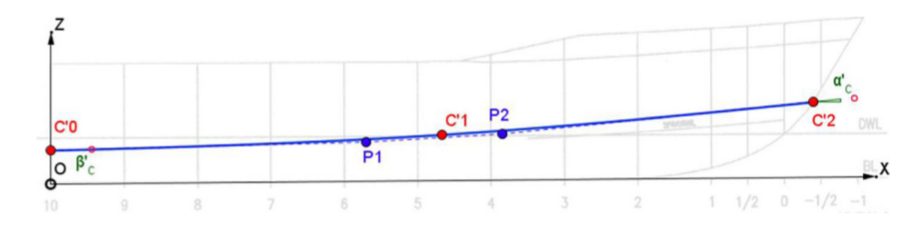
\includegraphics[width=9cm]{chineline}
\end{figure}
\end{frame}

%----------------------------------------------
\begin{frame}{Vista Lateral - Central}
\begin{figure}[h]	
\centering
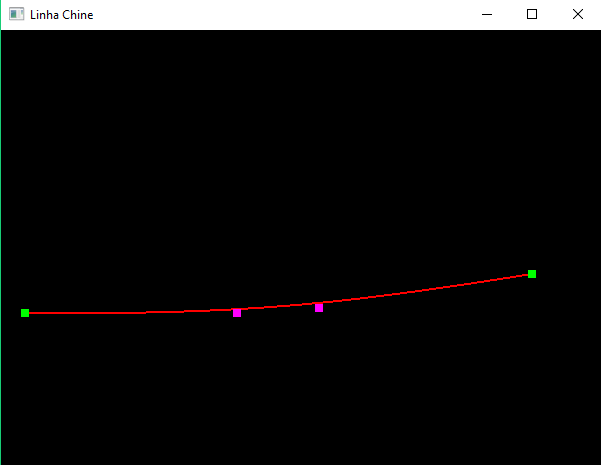
\includegraphics[width=9cm]{linhachine}
\end{figure}
\end{frame}
%----------------------------------------------
\begin{frame}{Vista Lateral - Completa}
\begin{figure}[h]	
	\centering
	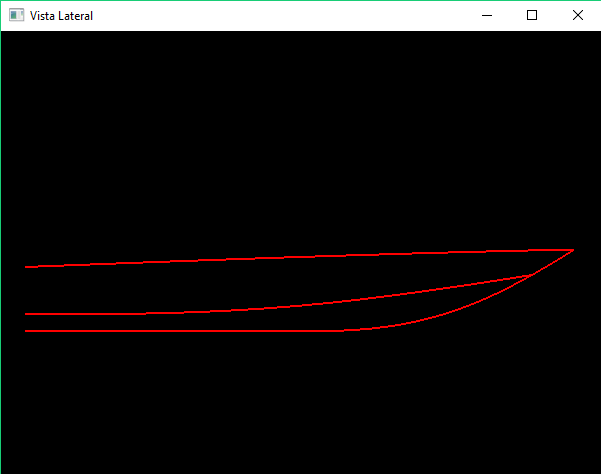
\includegraphics[width=9cm]{lateralopengl}
\end{figure}
\end{frame}
%----------------------------------------------
%----------------------------------------------
%----------------------------------------------
\subsection{Vista Superior}
\begin{frame}{Vista Superior}
\begin{itemize}
	\item Formada por 2 curvas principais:
	\begin{itemize}
		\item Linha \textit{Sheer}
		\item Linha \textit{Chine}
	\end{itemize}
\end{itemize}
\begin{figure}[h]
	\centering
	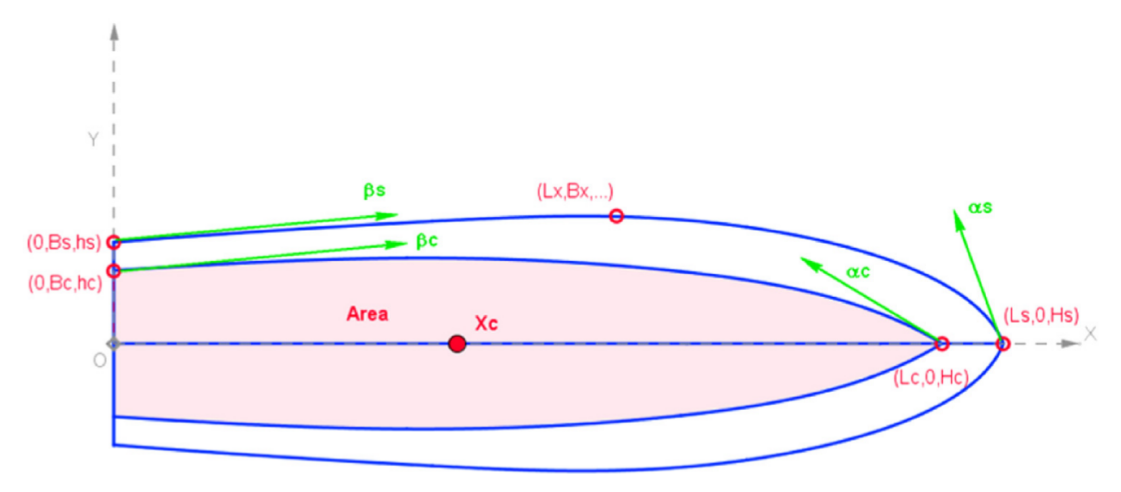
\includegraphics[scale=0.3]{vistasuperior}
	\caption{Exemplo Vista Superior}
	\label{fig:central}
\end{figure}
\end{frame}

%----------------------------------------------
\begin{frame}{Vista Superior - Sheer}
\begin{block}{Linha Sheer}
\begin{equation}
\centering
s_P(u) = B^3_0S_0 +B^3_1P_1 + B^3_2P_2 + B^3_3S_2
\end{equation}
\end{block}
\begin{itemize}
\item Restrições:
\begin{enumerate}
\item $s_P(0) = S_0$
\item $s_P(1) = S_2$
\item $s_P(u*) = S_X$
\item $s'_P(1) = tg(a_s)$
\end{enumerate}
\item Com as restrições acima podemos montar a matriz:
\end{itemize}
$
\begin{bmatrix}
	0 & $B'^3_1(u*)$ & 0 & $B'^3_2(u*)$ \\
	0 & 0 & $-tg(a_s)$ & 1 \\
	$B^3_1(u*)$ & 0 & $B^3_2(u*)$ & 0 \\
	0 & $B^3_1(u*)$& 0 &$B^3_2(u*)$
\end{bmatrix}
\begin{bmatrix}
	$XP_1$\\
	$ZP_1$\\
	$XP_2$\\
	$ZP_2$
\end{bmatrix}
=
\begin{bmatrix}
	$-B'^3_0(u*).B_s$\\
	$- tg(a_s).L_s$\\
	$Lx- B^3_3(u*)L_s$\\
	$Bx - B^3_0(u*).B_s$
\end{bmatrix}
$
\end{frame}

%----------------------------------------------
\begin{frame}{Vista Lateral - Sheer}
\begin{figure}[h]	
\centering
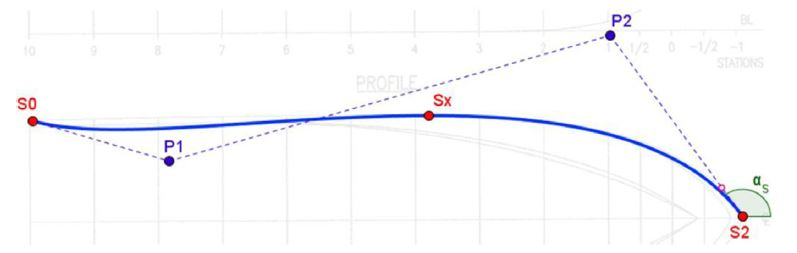
\includegraphics[width=9cm]{sheerlineplan}
\end{figure}
\end{frame}

%----------------------------------------------
\begin{frame}{Vista Lateral - Sheer}
\begin{figure}[h]	
\centering
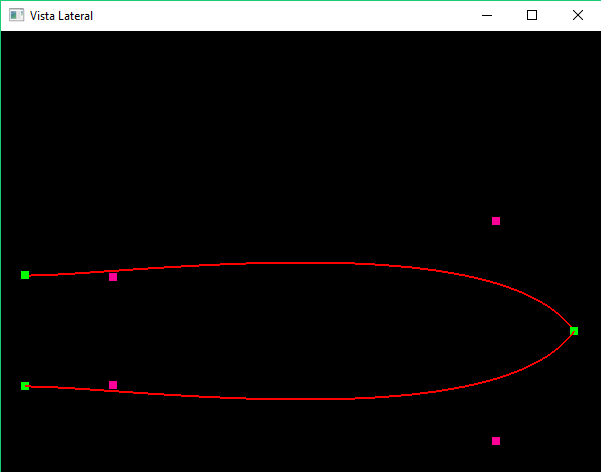
\includegraphics[width=9cm]{linhasheerplan}
\end{figure}
\end{frame}
%----------------------------------------------

\begin{frame}{Vista Superior - Chine}
\begin{block}{Linha Chine}
\begin{equation}
\centering
c_p(u) = B^3_0C_0 +B^3_1P_1+B^3_2P_2+B^3_3C_2
\end{equation}
\end{block}
\begin{itemize}
\item Restrições:
\begin{enumerate}
\item $c'_L(0) = tg(B_c)$
\item $c'_L(1) = tg(a_c)$
\item $c_L(u*) = C_1$
\end{enumerate}
\item Tal que $u* = \dfrac{Dist(K_0,K_1)^k}{Dist(K_0,K_1)^k + Dist(K_1,K_2)^k}$
\item Com as restrições acima podemos montar a matriz:
\end{itemize}
$	
\begin{bmatrix}
$-tg(B_c)$ & 1 & 0 & 0 \\
0 & 0 & $-tg(a_c)$ & 1 \\
$B^3_1(u*)$ & 0 & $B^3_2(u*)$ & 0 \\
0 & $B^3_1(u*)$& 0 &$B^3_2(u*)$
\end{bmatrix}
\begin{bmatrix}
$XP_1$\\
$ZP_1$\\
$XP_2$\\
$ZP_2$
\end{bmatrix}
=
\begin{bmatrix}
$L_c$\\
$B_c - tg(a_c).L_c$\\
$ B^3_3(u*)B_c$\\
$ B^3_0(u*).L_c$
\end{bmatrix}
$
\end{frame}
%----------------------------------------------
\begin{frame}{Vista Superior - Chine}
\begin{figure}[h]	
\centering
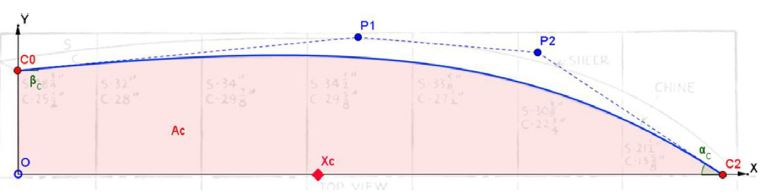
\includegraphics[width=9cm]{chinelineplan}
\end{figure}
\end{frame}

%----------------------------------------------
\begin{frame}{Vista Superior - Chine}
\begin{figure}[h]	
\centering
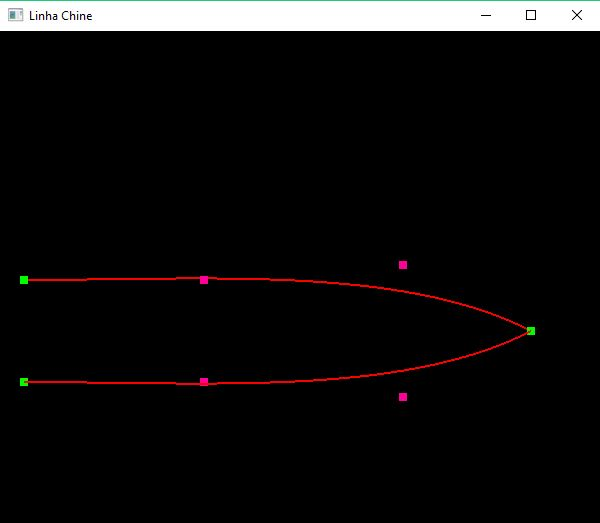
\includegraphics[width=9cm]{linhachineplan}
\end{figure}
\end{frame}
%----------------------------------------------
\begin{frame}{Vista Superior - Completa}
\begin{figure}[h]	
\centering
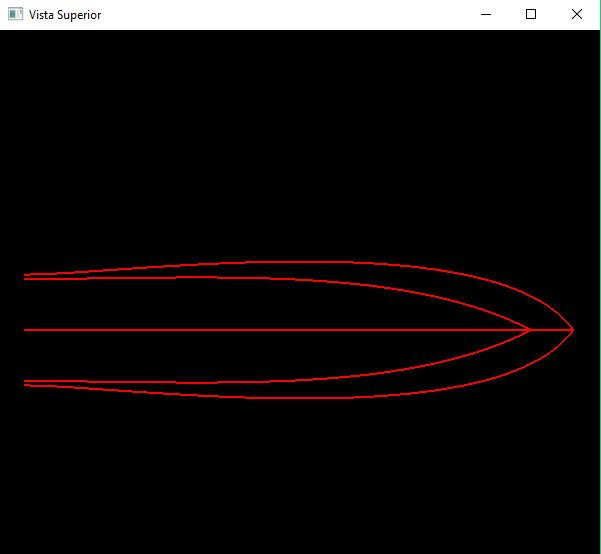
\includegraphics[width=9cm]{superioropengl}
\end{figure}
\end{frame}

\section{Trabalhos Futuros}
%----------------------------------------------
\begin{frame}
\tableofcontents[ 
    currentsubsection, 
    hideothersubsections, 
    sectionstyle=show/shaded
    ] 
\end{frame}
%-------------------------------------------------
\begin{frame}{Trabalhos Futuros}
\begin{itemize}
	\item Propor algoritmo evolutivo para a otimização de variáveis do projeto
	\item Implementar uma ferramenta computacional com interface amigável para auxiliar os projetistas desse tipo de embarcação.
	\item Sugerir modelos de embarcações otimizadas.
\end{itemize}

\end{frame}

%----------------------------------------------
\section{Cronograma}
%---------------------------------------------
\begin{frame}{Cronograma}
\begin{table}[ht]
\centering

%\caption{My caption}
\label{my-label}
\begin{tabular}{|l|l|}
\hline
\multicolumn{1}{|c|}{Mês} & \multicolumn{1}{c|}{Atividades}                                                                                                                                                    \\ \hline
Março                     & \begin{tabular}[c]{@{}l@{}}Desenvolvimento do casco 3D\\ Estudo dos parâmetros a serem otimizados\\Implementação do Algoritmo Genético\end{tabular}                                   \\ \hline
Abril                     & \begin{tabular}[c]{@{}l@{}}Implementar novos Operadores\\ Desenvolver Componentes Híbridos\end{tabular} \\ \hline
Maio                      & \begin{tabular}[c]{@{}l@{}}Desenvolvimento de Artigo\\ Desenvolvimento do software para \textit{plotagem} \\e otimização dos parâmetros\end{tabular}                               \\ \hline
Junho                     & \begin{tabular}[c]{@{}l@{}}Aperfeiçoar AGMO\\\end{tabular}                                                                                                 \\ \hline
Julho                     & Apresentação Final                                                                                                                                                                 \\ \hline
\end{tabular}
\end{table}
\end{frame}

\section{Bibliografia}
%----------------------------------------------
\begin{frame}{Referencial Bibliográfico}
\bibliographystyle{abbrv}

\bibliography{ahh}
\end{frame}
%---------------------------------------------
\begin{frame}
\titlepage
\end{frame}
%---------------------------------------------
\end{document}